% !TeX spellcheck = en_US
%\setcounter{chapter}{6} % set chapter counter so we begin at chapter 5
%\chapter{Laboration: PI/PID control of The Classroom Exo}


\section{Lab Introduction}

\begin{tcolorbox}[colback=blue!5!white,colframe=blue!75!black,title=Summary]
	In this chapter you will find the necessary documentation to setup your Classroom Exo, and try out the Force options. We have prepared some Lab exercises, to help you learn more about the force control options!
\end{tcolorbox}
\vspace{0.5cm}

An exoskeleton is a wearable mechanical structure that enhances or restores the physical abilities of the wearer by providing external support or amplification of movements \cite{AlTashi2024}. As the field of robotics grows leaps and bounds with every passing day as the world of STEM aims to integrate technology with humans to aid and support or enhance activities of daily living. Education leveraging these technologies has however been lacking. 
This lab is intended for use at a university level and is a derivative of a project aimed at converting an open-source exoskeleton into educational material \cite{AlTashi2024}. The Classroom Exo, the product that we will be using through the course of this lab, is a student-friendly optimized version of the EduExo Pro - An Advanced Robotic Exoskeleton Kit developed by Auxivo AG. 

\subsection{Risk section}
The Classroom Exo is not categorized as a medical device. Instead, its primary focus is educational. It is designed to provide hands-on experience with various control systems. There are some risks associated with the use of the Classroom Exo. Listed below are the potential risks, what has been done to prevent them, and the possible causes of these risks.
\begin{itemize}[]
	\item \textbf{Muscle fatigue:} Muscle fatigue can occur during prolonged use, as the Classroom Exo is somewhat heavy. To minimize this risk, an ergonomic design and proper usage guidelines have been implemented.
	\item \textbf{Injury risk:} The risk of injury is very low, but it still exists. The primary cause is misalignment between the Classroom Exo's mechanical joints and the user's shoulder and elbow joints. This risk has been minimized through proper calibration, an emergency stop feature, and clear instructions for how to put on the Classroom Exo.
\end{itemize}

\subsection{Learning objectives}
The goal of this lab is to provide hands-on experience with the Classroom Exo as a practical example of applying engineering principles within the biomedical field. Throughout the lab, you will explore how force sensors can be used to control an exoskeleton. By experimenting with different thresholding levels you will consider the practical applications of force-controlled exoskeletons, understanding how and why they are used in different scenarios. By the end of this lab you should be able to:

\begin{itemize}[]
	\item Implement force control on an exoskeleton and adjust threshold settings.
	\item Explain how threshold settings influence exoskeleton movement, and analyze its impact on performance and safety. 
	\item Evaluate the practical applications for this control method in terms of use case and user safety.	
\end{itemize}

\subsection{Prerequisite knowledge}
There is no specific prerequisite knowledge required for this lab. Any student group interested in product design, user safety, or gaining insight into biomedical engineering principles can benefit from this lab. However, due to the complexity of the system, the use of MATLAB, and potential troubleshooting, this lab may be most suitable for engineering students.

\subsection{Materials and methods}
For this lab, you will need a Bluetooth-enabled computer and MATLAB 2023b (although newer versions should also work). We will be interfacing with the exoskeletons using the “Updated BT-GUI” MATLAB application. Additionally, you will need one exoskeleton and a 2.5 and 3,0 Allen Key to adjust the arm length of the exoskeleton to fit the anatomy of the student who will be wearing the exoskeleton. 

\subsection{To do at home before the lab}
To make the most of the limited time you will have with the exoskeletons, you must come to the lab session well-prepared. Unforeseen issues or complications with the setup of the exoskeletons may arise, so proper preparation will ensure you have as much hands-on time as possible with the exoskeleton. Therefore before the lab asks you to:  
\begin{enumerate}[]
	\item Download MATLAB 2023b.
	\item Download the “Updated BT-GUI\_10-24”  folder from the GitHub link: \url{https://github.com/fabianjust/classroom-exo}
	\item Download and install the following MATLAB packages: 
	\begin{itemize}[]
		\item Control System Toolbox (version 23.2)
		\item Instrument Control Toolbox (version 23.2)
		\item Robotics System Toolbox (version 23.2)
		\item Sensor Fusion and Tracking Toolbox (version 23.2)
		\item Signal Processing Toolbox (version 23.2)
		\item Symbolic Math Toolbox (version 23.2)
	\end{itemize}
	\item Read the lab PM thoroughly.
\end{enumerate}


\newpage

\section{Introduction to the Exoskeleton}
Exoskeletons are increasingly being incorporated into rehabilitative settings, such as walking assists for people who have undergone spinal cord injuries, strokes, etc., in physiotherapy, and occupational therapy \cite{Hill2017}. Although aimed to be used in educational settings only, the Classroom Exo is an exoskeleton connected to the upper part of the body, over the shoulder, and the upper and lower arm, with a spring support to help lift the arm \autoref{fig:fig02}. Programmed on Arduino, it has three control systems - proportional–integral–-derivative controller (PID Controller), Electromyography signals from the muscles, and a force sensor on the wrist, the software of which is accessible as open-source, with a classroom-friendly graphical interface implemented on MATLAB. 

\begin{figure}[H]
	\centering
	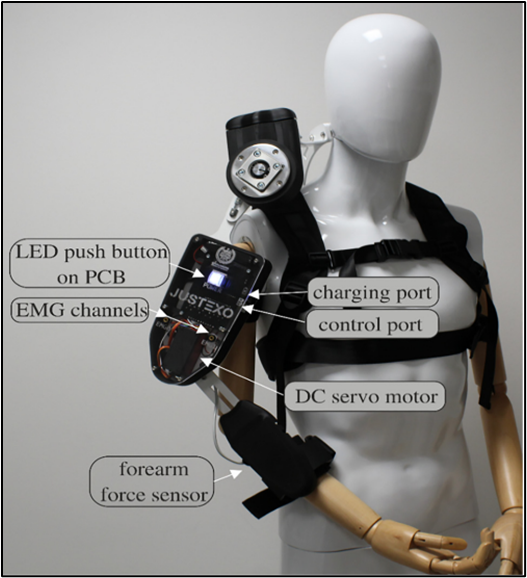
\includegraphics[width=0.7\linewidth]{img/fig_02}
	\caption{The Classroom Exo and its adaptations from EduExo Pro }
	\label{fig:fig02}
\end{figure}

\subsection{Setting up the Classroom Exo}
While putting on the exoskeleton it is helpful if one person holds it up and another tightens the straps.
\begin{enumerate}[]
	\item Put on the vest and fasten the buckles. 
	\item Make sure that the shoulder part of the exoskeleton is aligned with your shoulder, which can be seen in \autoref{fig:fig03}. And then tighten the chest and waist straps.
\end{enumerate}

\begin{figure}[H]
	\centering
	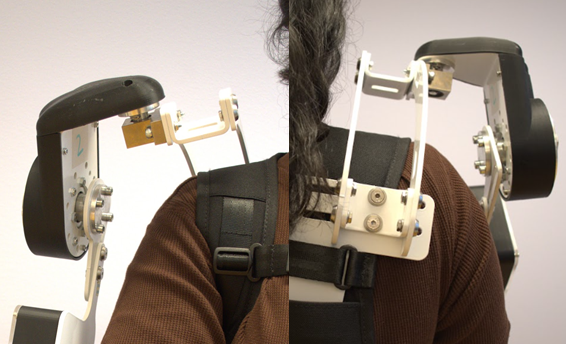
\includegraphics[width=0.4\linewidth]{img/fig_03}
	\caption{Shoulder joint aligned (left) and misaligned (right).}
	\label{fig:fig03}
\end{figure}

\begin{enumerate}[]
	\setcounter{enumi}{2}
	\item Tighten the straps around the elbow and the wrist and check alignment with the elbow joint according to \autoref{fig:fig04}. 
\end{enumerate}

\begin{figure}[H]
	\centering
	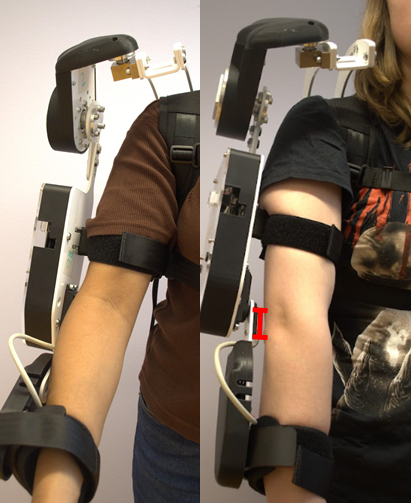
\includegraphics[width=0.4\linewidth]{img/fig_04}
	\caption{Correct alignment of elbow joint (left) and incorrect alignment (right), misalignment marked in red.}
	\label{fig:fig04}
\end{figure}

\begin{enumerate}[]
	\setcounter{enumi}{3}
	\item If the Classroom Exo has the correct joint alignment as seen in figure 4 and 3, proceed to section 2.1.2. If not, proceed with section 2.1.1 “Adjusting the exoskeleton”.
\end{enumerate}

\subsubsection{Adjusting the exoskeleton}
To be able to adjust the arm length of the Classroom Exo, a 2.5 and 3.0 Allen Key is needed.

\begin{enumerate}[]
	\item Under the shoulder joint on the back of the exoskeleton you can find two bolts for which the 3.0 Allen Key fits, the bolts are marked in \autoref{fig:fig05}. Loosen these, align shoulder joints according to \autoref{fig:fig03} and tighten the bolts. 
\end{enumerate}



\begin{figure}[H]
	\centering
	\begin{center}
		\begin{tikzpicture}
			\node(a){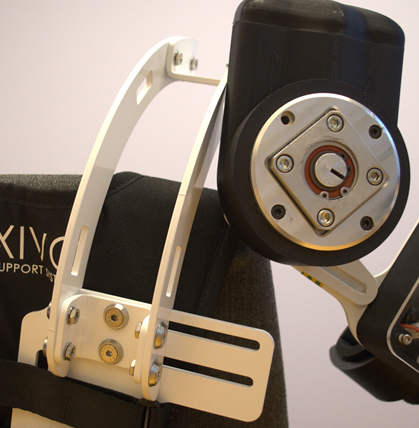
\includegraphics[width=0.4\linewidth]{img/fig_05}};
			\node at(a.center)[draw, red,line width=3pt,circle, minimum width=45pt, minimum height=45pt,rotate=-40,yshift=-65pt]{};
		\end{tikzpicture}   
	\end{center}
	\caption{Bolts for adjusting shoulder breadth in red.}
	\label{fig:fig05}
\end{figure}



\begin{enumerate}[]
	\setcounter{enumi}{1}
	\item To align the elbow, loosen the bolts on the inside of the shoulder joint illustrated in \autoref{fig:fig06}. Use the 3.0 Allen key to do this. Slide the arm such that the elbow joint of the exoskeleton and the user is aligned such as in \autoref{fig:fig04}. Tighten the bolts.
\end{enumerate}

\begin{figure}[H]
	\centering
	\begin{center}
		\begin{tikzpicture}
			\node(a){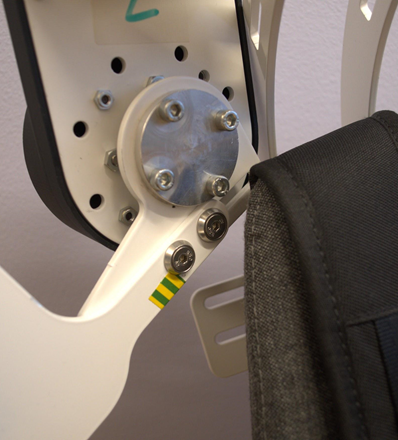
\includegraphics[width=0.4\linewidth]{img/fig_06}};
			\node at(a.center)[draw, red,line width=3pt,circle, minimum width=45pt, minimum height=45pt,rotate=0,yshift=-7pt, xshift=-1pt]{};
		\end{tikzpicture}   
	\end{center}
	\caption{Bolts to adjust upper arm length for elbow alignment marked in red.}
	\label{fig:fig06}
\end{figure}



\begin{enumerate}[]
	\setcounter{enumi}{2}
	\item To adjust the position of the wrist cuff, loosen the bolt on the lower part on the arm of the exoskeleton marked in \autoref{fig:fig07}, using the 2.5 Allen key. Adjust length and tighten the bolts.
\end{enumerate} 

\begin{figure}[H]
	\centering
	\begin{center}
		\begin{tikzpicture}
			\node(a){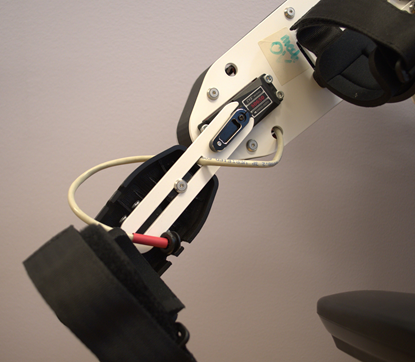
\includegraphics[width=0.4\linewidth]{img/fig_07}};
			\node at(a.center)[draw, red,line width=3pt,circle, minimum width=15pt, minimum height=15pt,rotate=0,xshift=-12pt, yshift=-2pt]{};
		\end{tikzpicture}   
	\end{center}
	\caption{Bolts to adjust lower arm length for positioning of wrist cuff marked in red.}
	\label{fig:fig07}
\end{figure}
\subsubsection{Connecting to the device and starting the GUI}
\begin{enumerate}[]
	\item Turn on the exoskeleton by pushing the “LED push button on PCB” as seen in \autoref{fig:fig08}. It  should blink blue indicating that it is searching for a Bluetooth device.
	\item When you are connecting to the exoskeleton for the first time, go to your computer's Bluetooth settings and add a Bluetooth device. When pairing, the name of your device will be XX\_CLASSROOM\_EDU\_EXO\_PRO where the XX is a number between 01 to 08 depending on which exoskeleton you have.
\end{enumerate}

\begin{figure}[H]
	\centering
	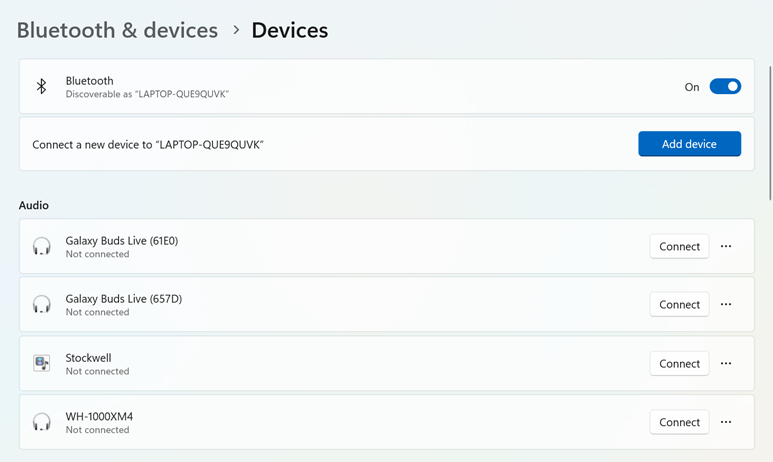
\includegraphics[width=0.7\linewidth]{img/fig_08}
	\caption{Pairing to a Bluetooth device for the first time.}
	\label{fig:fig08}
\end{figure}
\begin{enumerate}[]
	\setcounter{enumi}{2}
	\item In your computer's display settings set the screen size to 100\%.
\end{enumerate}
\begin{figure}[H]
	\centering
	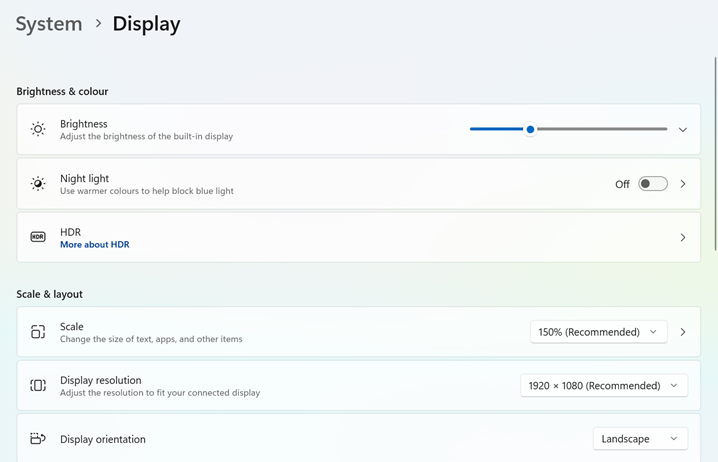
\includegraphics[width=0.7\linewidth]{img/fig_09}
	\caption{Changing screen sizing.}
	\label{fig:fig09}
\end{figure}

\begin{enumerate}[]
	\setcounter{enumi}{3}
	\item Open MATLAB, locate the BT\_GUI file and double click on it. Or locate the file in your file explorer and select open with MATLAB. If you open the file in MATLAB’s app designer, click run.
	\item When the GUI is opened, choose the correct Bluetooth device, and click connect. 
\end{enumerate}

\begin{figure}[H]
	\centering
	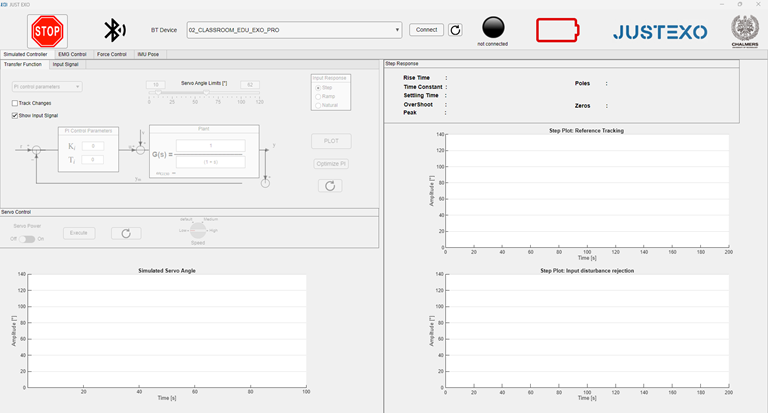
\includegraphics[width=0.7\linewidth]{img/fig_10}
	\caption{Connecting to the Bluetooth device.}
	\label{fig:fig10}
\end{figure}

The power button on the exoskeleton and the indicator in the GUI should change color to either green, yellow or red depending on the battery level.


\newpage
\section{Force controller}
\subsection{Introduction}



Force control enables systems to detect and respond to external forces, making them adaptable to environmental changes or user force input \cite{Falkowski2024}. This concept is widely used across engineering, from rehabilitation to industrial applications \cite{Lang2022}. In rehabilitation, exoskeletons use force control to either assist in or add resistance to patients' intended motions \cite{Falkowski2024}. By using exoskeletons we can allow for movements that the patient otherwise could not perform, avoid over-extension, relieve physiotherapists' work burden, and gradually reduce the assistance as the patient regains strength \cite{Falkowski2024, Dickmann2021}.

Additionally, it might be useful in industrial settings for workers where the motor in the exoskeleton helps them in movements when the sensors detect forces or strains that would otherwise be harmful to the worker's body, thus preventing injuries \cite{Golabchi2022}. 

The Classroom Exo uses strain gauges at the wrist cuff to detect forces, see \autoref{fig:fig02}. When these sensors experience deformation due to a force, they change their resistance, altering the voltage over them \cite{AlTashi2024}. These sensors allow the exoskeleton to detect a voltage difference when an upward force exceeds a threshold and subsequently flex the elbow joint. Similarly, exceeding a downward threshold causes the elbow joint to extend, moving the arm to a straighter position.

\subsection{Force controller setup}
The exoskeleton should be put on before starting this part.

1.	Choose the “Force control” tab, and then the “Threshold” tab, which can be seen in \autoref{fig:fig11}.



\begin{figure}[H]
	\centering
	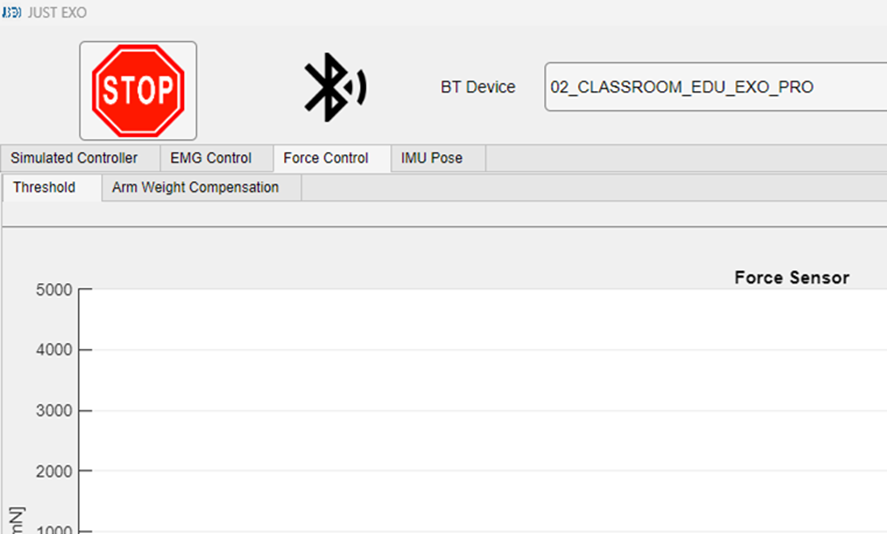
\includegraphics[width=0.7\linewidth]{img/fig_11}
	\caption{Choosing the force control tab (red) and the threshold tab (blue).}
	\label{fig:fig11}
\end{figure}



2.	At the bottom of the tab, you can see the force control parameters. Where you can change the upper and lower threshold force limits, the servo motor speed, and the applied filter. See \autoref{fig:fig12}.

\begin{figure}[H]
	\centering
	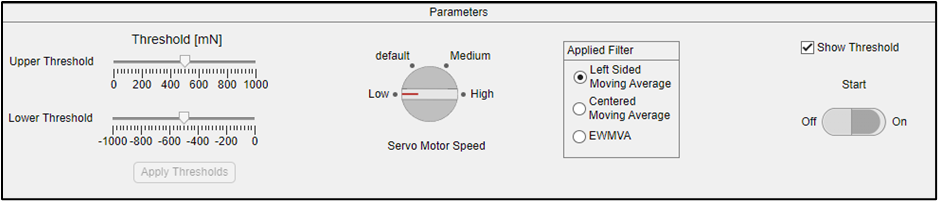
\includegraphics[width=0.7\linewidth]{img/fig_12}
	\caption{The tunable force control parameters.}
	\label{fig:fig12}
\end{figure}

3.	Ensure the “show threshold” box which you can see in \autoref{fig:fig12} is checked to see when the force on the wrist cuff exceeds the upper or lower threshold. 
4.	Click start. When trying out the force control by flexing and extending your arm you should see something like this:
 

\begin{figure}[H]
	\centering
	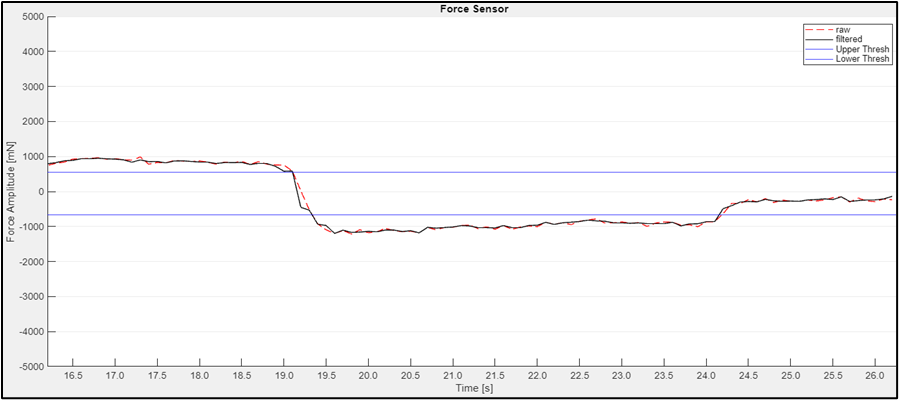
\includegraphics[width=0.7\linewidth]{img/fig_13}
	\caption{Force sensor data.}
	\label{fig:fig13}
\end{figure}

5.	When changing the threshold values, make sure to click “apply thresholds” and turn the start button off and then on again. 


\newpage
\subsection{Exercises}

\begin{tcolorbox}[colback=red!5!white,colframe=red!75!black,title=Attention]
	\textbf{OBS!} You can break pieces of the exoskeleton. Don’t try to exceed thresholds by more than necessary.
\end{tcolorbox}
\vspace{0.5cm}



This section outlines a series of exercises to be completed during the allotted lab time. These exercises are designed to deepen your understanding of how Force control can be applied in combination with the Classroom Exo. The results of the exercises must be documented in a separate report. The question exercises are meant to be discussed within a group.

\subsubsection{Default sensitivity}

Test the default threshold settings (lower threshold = -500 mN, upper threshold = 500 mN) to understand what force control feels like. 

\paragraph{Tasks:}
\begin{enumerate}[]
	\item Flex your bicep to exceed the higher threshold and see how the elbow joint flexes. 
	\item Try to straighten your arm, exerting force in the other direction exceeding the lower threshold causing the joint to straighten. 
\end{enumerate}
	
\paragraph{Question:} 	
\begin{enumerate}[]
	\item Is there a maximum and minimum angle of the elbow flexion and how does this play into user safety?
\end{enumerate}
 
\subsubsection{Rehabilitation scenario}
To simulate a rehabilitation scenario we will now increase the sensitivity of the system. 

\paragraph{Tasks:}
\begin{enumerate}[]
	\item Set the lower threshold value to -100, and set the upper threshold to 100.
	\item Now try to flex your arm and extend it. How is it different from the default threshold settings? 
\end{enumerate}

\paragraph{Questions:} 
\begin{enumerate}[]
	\item In what real-life use-cases for exoskeletons would there be for high-sensitivity sensing of forces?
	\item Experiment with different thresholds. Can you find a usable threshold for the use case you thought of? If you couldn’t find a usable threshold, why? 
	\item In a rehabilitation setting, how can lower versus higher sensitivity affect the users in terms of support and safety?
	\item Are there any other safety risks in this use case?
\end{enumerate}

\subsubsection{Worker scenario}
In this section, we will simulate an industrial worker as a user by setting the thresholds so we have a low-sensitivity system. 

\paragraph{Tasks:}
\begin{enumerate}[]
	\item Try setting the lower threshold to a higher setting and the upper threshold to a lower value. A suggestion would be to set the lower threshold to a value close to -1000, and the upper threshold to 1000.
	\item Test it out, what does it feel like? 
\end{enumerate}	

\paragraph{Questions:} 
\begin{enumerate}[]
	\item In what real-life use cases for exoskeletons would there be for low-sensitivity sensing of forces? 
	\item Experiment with different thresholds, which ones do you think work best for this scenario and why? If you couldn’t find a usable threshold, why? 
	\item How does a lower versus higher sensitivity affect the users in this use case in terms of support and safety in this use case?
	\item Are there any other safety risks in this use case?
\end{enumerate}

\subsubsection{Servo speed}
We will now experiment with servo speed and reflect on the uses. 

\paragraph{Tasks:}
\begin{enumerate}[]
	\item Set the speed to low, medium, and then high.
	\item 	Test it out, what does it feel like?
\end{enumerate}

	
\paragraph{Questions:} 
\begin{enumerate}[]
	\item What would be the benefit or drawback of having a static servo speed? 
	\item What would be the benefit or drawback of having a dynamic servo speed? 
	\item Reflect on this in terms of use case and safety. 
\end{enumerate} 	

\subsection{Discussion}
For the best learning experience, feel free to discuss the results your group obtained from each step between groups to gain understanding and new perspectives.
\begin{enumerate}[]
	\item What differed between your answers and the answers of other groups?
	\item Why did your answers or conclusions differ?
	\item Did your discussions between groups lead to new insights or ideas? If so, what were they?
\end{enumerate} 	


\section{Typical errors and Troubleshooting}
In this section, we present typical errors and issues encountered during testing of the Classroom Exo. 
\begin{enumerate}[]
	\item If you experience that the exoskeleton arm switches between extending and contracting, almost vibrating, it might be because the upper and lower thresholds are too close to each other. 
	\item If the thresholds are not showing or the signal is not showing after changing the thresholds, then click “apply thresholds” and turn the start button off and then on again. Wait for the signal to appear.
\end{enumerate} 

\begin{tcolorbox}[colback=green!5!white,colframe=green!75!black,title=Hint]
	You can find a more comprehensive Troubleshooting documentation in the Manual on our GitHub!
\end{tcolorbox}
\vspace{0.5cm}







